\documentclass{article}
\usepackage{graphicx} % Required for inserting images
\usepackage{tabularx}
\usepackage{amsmath}
\usepackage[T2A]{fontenc}
\usepackage[top=5cm,bottom=3cm,right=3cm,left=3cm]{geometry}

\title{Анализ программ - Lab2}
\author{Матвей Русаков m.rusakov@innopolis.university SD-03}
\date{Апрель 2025}

\begin{document}

\maketitle


\section*{Предисловие}

Материал и скриншоты из гидры я разместил на GitHub, в директории Lab2/lab\_data/ вы можете найти исходник, скриншоты и сишный код мейн функции для каждой из задач

\section*{Task 0}

\paragraph{Мейн функция} нулевой задачи выглядит вот так:

\begin{verbatim}
undefined8 FUN_00101170(void)

{
  int iVar1;
  char *__s1;
  
  __s1 = (char *)malloc(400);
  printf("%s","Hello, enter the flag:\n");
  __isoc99_scanf(&DAT_00102004,__s1);
  iVar1 = strcmp(__s1,"flag{6057f13c496ecf7fd777ceb9e79ae2 85}");
  if (iVar1 == 0) {
    printf("%s",&DAT_00102046);
  }
  else {
    printf("%s","TRY HARDER");
  }
  return 0;
}

\end{verbatim}

\paragraph{Описание}
\paragraph{}
Данный код --- это функция на языке C, реализующая проверку флага. Опишем её по шагам:

\begin{enumerate}
    \item Выделяется память под строку:
    \begin{verbatim}
    __s1 = (char *)malloc(400);
    \end{verbatim}
    Здесь выделяются 400 байт для хранения пользовательского ввода.

    \item Печатается приглашение пользователю:
    \begin{verbatim}
    printf("%s", "Hello, enter the flag:\n");
    \end{verbatim}
    На экран выводится сообщение:
    \begin{verbatim}
    Hello, enter the flag:
    \end{verbatim}

    \item Считывается ввод:
    \begin{verbatim}
    __isoc99_scanf(&DAT_00102004, __s1);
    \end{verbatim}

    \item Введённая строка сравнивается с жёстко закодированным флагом:
    \begin{verbatim}
    iVar1 = strcmp(__s1, "flag{6057f13c496ecf7fd777ceb9e79ae285}");
    \end{verbatim}
    Если строки совпадают (iVar1 == 0), выполняется блок if, иначе --- else.

    \item Условие:
    \begin{verbatim}
    if (iVar1 == 0) 
        printf("%s", &DAT_00102046);
    else
        printf("%s", "TRY HARDER");
    \end{verbatim}
    Если строка верная, выводится сообщение по адресу \&DAT\_00102046 (строка "WIN"), иначе выводится сообщение "TRY HARDER".

    \item Функция возвращает 0:
    \begin{verbatim}
    return 0;
    \end{verbatim}
\end{enumerate}

\noindent
\paragraph{Особенности}
\begin{itemize}
    \item Отсутствует освобождение памяти после \texttt{malloc} (утечка памяти);
    \item Формат ввода не позволяет вводить пробелы (если используется \%s);
    \item Сравнение производится напрямую, без шифрования или дополнительных преобразований.
\end{itemize}

\newpage
\paragraph{Тестовые запуски}
\paragraph{}
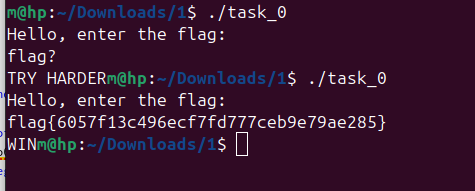
\includegraphics[width=0.7\linewidth]{static/solution_task_0.png}


\section*{Task 1}
\paragraph{Как выглядит мейн функция} - вы можете найти на гитхабе в референсах. Она слишком длинная, чтобы записывать ее в репорт
\paragraph{Описание}

Данный код --- это функция на языке C, которая реализует проверку флага, аналогичную предыдущей, но с поэтапной посимвольной проверкой. Опишем её по шагам:

\begin{enumerate}
    \item Объявление локальных переменных и инициализация:
    \begin{verbatim}
    int iVar1;
    int local_40;
    int local_3c;
    char local_38 [4];
    char cStack_34;
    char cStack_33;
    ...
    char acStack_13 [7];
    undefined4 local_c;
    
    local_c = 0;
    local_3c = 0;
    \end{verbatim}

    \item Приветственное сообщение:
    \begin{verbatim}
    printf("%s",
      "Hello, this task is very similar to the previous one, but has  some modifications\nenter the flag:\n"
    );
    \end{verbatim}
    Выводит сообщение с просьбой ввести флаг.

    \item Чтение посимвольного ввода (38 символов):
    \begin{verbatim}
    for (local_40 = 0; local_40 < 0x26; local_40 = local_40 + 1) {
      __isoc99_scanf(&DAT_00102069, local_38 + local_40);
    }
    \end{verbatim}

    \item Пошаговое посимвольное сравнение (каждый символ сравнивается отдельно через \texttt{strncmp}), например:
    \begin{verbatim}
    iVar1 = strncmp("f", local_38, 1);
    if (iVar1 == 0) {
      local_3c = 1;
      iVar1 = strncmp("l", local_38 + 1, 1);
      if (iVar1 == 0) {
        local_3c = 2;
        iVar1 = strncmp("a", local_38 + 2, 1);
        if (iVar1 == 0) {
          local_3c = 3;
          ...
    \end{verbatim}

    Проверка продолжается символ за символом:
    \begin{verbatim}
    ...
    iVar1 = strncmp("}", acStack_13, 1);
    if (iVar1 == 0) {
      local_3c = 0x26;
    }
    \end{verbatim}

    \item Финальная проверка:
    \begin{verbatim}
    if (local_3c == 0x26) {
      printf("%s", &DAT_00102097);
    }
    else {
      printf("%s", "TRY HARDER");
    }
    \end{verbatim}

    \item Возврат из функции:
    \begin{verbatim}
    return 0;
    \end{verbatim}
\end{enumerate}

\paragraph{Отличия и особенности}
\begin{itemize}
    \item task\_0 считывает строчку - после enter или пробела запустится скрипт дальше, в то время как в task\_1 используется посимвольный ввод

    \item Поскольку флаг состоит из 38 символов, функция будет ждать, пока пользователь не введет 38 символов и только потом запустит дальше

    \item В task\_1 последовательное, посимвольное сравнение с буквами из правильного флага

    \item Флаг для этой задачи немного другой - "flag{444Y0urB4seRBe803g2Usdfd4ds9y1re}"
\end{itemize}

\paragraph{Тестовые запуски}
\paragraph{}

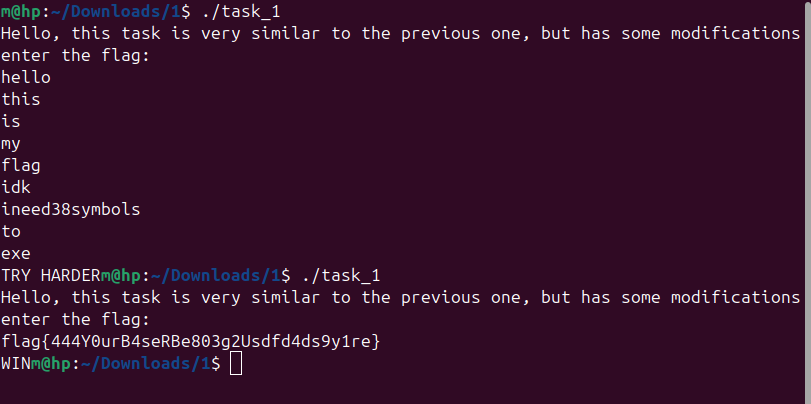
\includegraphics[width=0.75\linewidth]{static/solution_task_1.png}

\end{document}
